\chapter{Introduction}

\section{Assignment BEM }

This group assignment is the anbalysis of a Wind Turbine rotor's performance. The methodology implemented to estimate the performance is the Blade Element Moment theory. The BEM theory is a powerfull procedure used to compute quick and cheap the main flow characteristics. It is way simpler to implement and solve compared to other alternatives such as CFD. This is one of the main reasons why the BEM is a widely used tool to estimate the rotor performance in the Wind Energy business. \\

This is an introduductory study and therefore uses a simplified wind turbine model. The rotor specifications are provided in Table \ref{Rot_specs} and the operation regimes are stated in Table \ref{Op_specs}.

\begin{table} [htbp]
\centering
\caption{Rotor design parameters}
\begin{tabular}{|l|l|} 
\hline
\textbf{Rotor parameter}    & \textbf{Specification}                             \\ 
\hline
Radius                      & 50 m                                               \\ 
\hline
Number of blades            & 3                                                  \\ 
\hline
Blade start                 & 0.2 r/R                                            \\ 
\hline
Twist                       & 14*(1-r/R)~~~~ (for r/R0.2)                       \\ 
\hline
Blade pitch                 & -2 degrees                                         \\ 
\hline
Chord distribution function & (3*(1-r/R)+1) m~~~~ (for r/R\textgreater{}0.2)   \\ 
\hline
Airfoil                     & DU 95-W-180                                        \\
\hline
\end{tabular}
\label{Rot_specs}
\end{table}  

\begin{table}[htbp]
\centering
\caption{Operational regime specifications}
\begin{tabular}{|l|l|} 
\hline
\textbf{Operational parameter} & \textbf{Specification}  \\ 
\hline
$U_{\infty}$                    & 10 m/s                  \\ 
\hline
TSR  ($\lambda$)                   & 3                       \\ 
\hline
Yaw angles                     & 0, 15 and 30 degrees    \\
\hline
\end{tabular}
\label{Op_specs}
\end{table}


\section{Single polar innacuracies}

This study would have some innacuracies as it is planned if it is compared to a modern commercial wind turbine. One of the most relevant innacuracies is the fact that the aerodynamics coefficients in all the radial sections of the blade have been extracted from the same polar curve. \\

Firstly, using single polar means assuming that all the radial positions are operating at the same Reynolds number. This is most probably false. Because from the Reynolds definition:
\begin{equation}
Re = \frac{ W \cdot c}{\nu}
\end{equation}
It has to be considered that as a first aproximation that the relative velocity perceived by the airfoil at each section is depending on the radius. The relative velocity can be estimated like:
\begin{equation}
W = \sqrt{(U_\infty \cdot (1-a) )^2 + (\Omega \cdot r (1+a'))^2}
\end{equation}
While the chord distrubution is ruled by the equation:
\begin{equation}
c = 3 \cdot (1-\mu) + 1 
\end{equation}
Then the Reynolds can be expressed as:
\begin{equation}
\text{Re} \quad Re(\mu)=\frac{\sqrt{(U_\infty*(1-a))^2 + (\lambda \cdot U_\infty \cdot \mu \cdot (1+a'))^2} \cdot c(\mu) } {\nu}\, [-]
\end{equation}
Then, as an example it is extracted the maximum and minimum Reynolds values from a BEM calculation at TSR = 8 with the converged inductions for the velocity. These sections are would have a chord
\begin{equation}
\text{Blade root chord} \quad c(0.208)=3 \cdot (1-0.208)+1=3.376 \, \text{m}
\end{equation}
\begin{equation}
\text{Blade tip chord} \quad  c(0.672)=3 \cdot (1-0.672)+1= 1.984 \, \text{m}
\end{equation}
While the Reynolds would be.
\begin{equation}
\text{Root Re} \quad Re(0.208)= \frac{\sqrt{(10*(1-a))^2 + (8 \cdot 10 \cdot 0.208 \cdot (1+a'))^2} \cdot c (0.208) } {\nu} \, = 4.47 \cdot 10^6
\end{equation}
\begin{equation}
\text{Max Re} \quad Re(0.672)= \frac{\sqrt{(10*(1-a))^2 + (8 \cdot 10 \cdot 0.672 \cdot (1+a'))^2} \cdot c (0.672) } {\nu} \, = 7.63 \cdot 10^6
\end{equation}

Usually the increase in relative velocity along the blade is higher than the decrease in chord. Hence, the Reynolds number will be larger close to the tip, which usually means improving the aerodynamic coefficients performance.  \\

Secondly, there are several models proposed as the one wrriten by Snel et al. making reference to correction model of the polar data caused by the 3D effects. In particular, the one propsoed by Snel states that it appears a delay in the stall of the sections closer to the root where the relative velocity is smaller. The Snel corection is modeled like eq (1
3.190) in the Wind Energy Handbook. 
\begin{equation}
C_{L_{3D}} = C_{L_{2D}} + 3 \cdot (\frac{c}{r})^2 \cdot \Delta C_L
\end{equation}
This was initially pointed out by Himmelskamp, who observed in propellers \cite{weh-ch3} \textit{"lift coefficients being attained at the inboard section of a rotating blade which are significantly in excess of the maximum value possible in two-dimensional static tests."} Figure \ref{snel} is provided to show approximately the order of magniude that this kind of correction might have on the power output. Rotational effects could have been taken into account in this study by using different airfoil polars depending on the blade section. Alternatively, it is also possible to include the 3D correction equations to the BEM code when extracting the aerodynamics coefficient from the polar files, but it seems a less efficient procedure.\\

\begin{figure}[htbp]
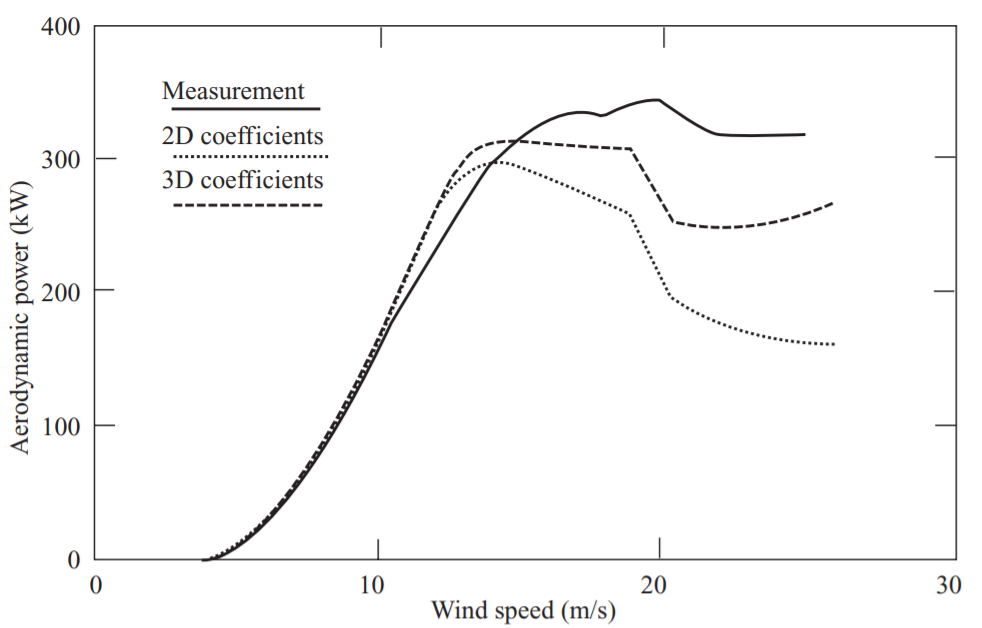
\includegraphics[width=0.75\textwidth]{./img/snel_fig.png}
\caption{ Snel 3D correction example, extracted from \cite{weh-ch3} \textit{A Comparison of Measured and Snel’s Predicted Power Curves for a NORTANK 300 kW Turbine}}
\centering
\label{snel}
\end{figure}

And lastly, it is not an strict inaccuracy, but nowadays wind trubine designs tend to optimize the structural and aerodynamics performance of a rotor. And to achieve that goal it is common to use different airfoils along the blade, which would yield different polar curves, as opposed to this study. Therefore it would be closer to the optimal to use slender airfoils near the tip to maximixe the aerodynamic performance and thicker airfoils closer to the root in order to increase their stiffness and load-carrying capacity. 